\section{Results}
% What we accomplihesd, everything which we created, invented, etc. should preferentially go here.
% Descriptive, opinions either absent, or as objective-ish comments when facts are stated.
% Should, could, might, etc. sparingly and ideally not here but in discussion.


\subsection{Repository Structure}

In order to improve the reexecution reliability of the OPVFTA article we have constructed a parent repository which leverages Git and DataLad to link all reexecution requirements.
This framework uses Git submodules for resource referencing, and DataLad \cite{datalad} in order to permit Git integration with data resources.

These submodules include the original article, the raw data it operates on, and a reference mouse brain templates package.
Additionally, the top-level repository directly tracks the code required to coordinate the OPFVTA article reexecution and subsequent generation of \emph{this} article.
The code unique to the reexecution framework consists of container image generation and container execution instructions, as well as a Make system for process coordination (\cref{fig:topology}).
This repository structure enhances the original reference article by directly linking the data at the repository level, as opposed to relying on its installation via a package manager.
Notably, however, the article source code itself is not duplicated or further edited here, but handled as a Git submodule, with all proposed improvements being recorded in the original upstream repository.
The layout constructed for this study thus provides robust provenance tracking and constitutes an implementation of the YODA principles (a recursive acronym for “YODAs Organigram on Data Analysis” \cite{yoda}).

The Make system is structured into a top-level Makefile, which can be used for container image regeneration and upload, article reexecution in a containerized environment, and meta-article production.
There are independent entry points for both \emph{this} and the original article — making both articles reexecutable (\cref{fig:workflow}).
Versioning of the original article reexecution is done via file names (as seen in the \texttt{outputs/} subdirectories of \cref{fig:topology}) in order to preserve shell accessibility to what are equivalent resources.
Versioning of the meta-article is handled via Git, so that the most recent version of the work is unambiguously exposed.

The meta-article targets redirect to a Makefile in the \texttt{article/} subdirectory, which contains this document's human-readable text in \TeX{} format, alongside scripts for generating dynamical elements based on the reexecution results seen in the \texttt{outputs/} directory.
The original article reexecution is provided by two alternative targets, using either the Open Container Initiative standard, or Singularity.
Both original article reexecution targets wrap the \texttt{produce\_analysis.sh} script, which is a thin compatibility layer accessing the Make system of the original article.
This alternative is introduced in order to assess feasibility as well as potential variability across virtualization infrastructures.


\begin{figure*}
	\centering
	\includegraphics[clip,width=0.99\textwidth]{figs/topology.pdf}
	\caption{
		\textbf{The directory topology of the new reexecution system nests all resources and includes a Make system for process coordination.}
		Depicted is the directory tree topology of the repository coordinating OPFVTA reexecution.
		Nested directories are represented by nested boxes, and Git submodules are highlighted in orange.
		The article reexecution PDF results are highlighted in light green, and the PDF of the resulting meta-article (i.e. this article) is highlighted in light blue.
	}
	\label{fig:topology}
\end{figure*}


\begin{figure*}
	\centering
	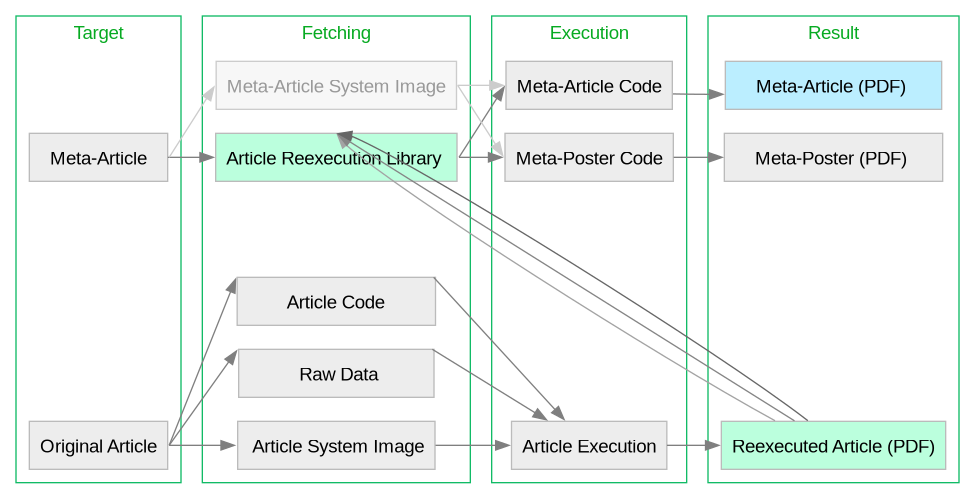
\includegraphics[clip,width=0.99\textwidth]{figs/workflow.pdf}
	\caption{
		\textbf{The reexecution system encompasses both the Original Article and Meta-Article as independent Make targets.}
		Depicted is the reexecution system workflow, with two reexecution entry points, the “Original Article and the “Meta-Article” (i.e. \textit{this} article, which also performs the reproduction assessment).
		Notably, for the generation of the meta-article, the Original Article can be executed, or not — the meta-article will dynamically include all reexecution results which are published, as well as all which are locally produced.
		The article reexecution PDF results are highlighted in light green, and the PDF of the resulting meta-article (i.e. this article) is highlighted in light blue.
		Optional nodes (such as fetching a container image for meta-article reexecution) are faded gray.
	}
	\label{fig:workflow}
\end{figure*}


\subsection{Resource Refinement}

As a notable step in our article reproduction effort, we have updated resources previously only available as tarballs (i.e. compressed \texttt{tar} archives), to DataLad.
This refinement affords both the possibility to cherry-pick only required data files from the data archive (as opposed to requiring a full archive download), as well as more fine-grained version tracking capabilities.
In particular, our work encompassed a re-write of the Mouse Brain Templates package \cite{mbt05} Make system.
In its new release \cite{mbt10}, developed as part of this study, Mouse Brain Templates now publishes tarballs, as well as DataLad-accessible unarchived individual template files.


\subsection{Best Practice Guidelines}

As part of this work we have contributed substantial changes to the original OPFVTA repository, based on which we formulate a number of best practice guidelines, highly relevant in the production of reexecutable research outputs.

\subsubsection{Errors should be fatal more often than not.}

By default, programs written in the majority of languages (including e.g. Python and C) will exit immediately when running into an unexpected operation.
The POSIX shell and other similar or derived shells, such as Bash and Zsh, behave differently.
Their default is to continue with execution of the next scripted command, and only exit with a non-zero code when the list of commands is exhausted or the \texttt{exit} command is called explicitly.
As a result, an execution of the script could continue for hours before it fails, and the original error message might be lost in the flood of output, making it hard or impossible to localize and address the original problem.
This behavior can be mitigated by prepending \texttt{set -e} to the respective shell script, which changes the default behavior so that execution is stopped as soon as a command exits with an error code.
Additionally, shell scripts treat undefined variables as a variable having an empty value, with empty values causing no errors.
This can lead to numerous ill-defined behaviors, including a command such as \texttt{rm -rf "\${PREFIX}/"} removing all files on the system if \texttt{PREFIX} is not defined.
This can be addressed by prepending \texttt{set -u} so that an error is raised and execution is stopped as soon as an undefined variable is referenced.
To summarize, we recommend including \texttt{set -eu} at the top of every shell script to guarantee it exits as soon as any command fails or an undefined variable is encountered.
This is in line with the “Fail Early” principle advocated in the ReproNim Reproducible Basics Module \cite{repronim:reprobasics}.

\subsubsection{Avoid assuming or hard-coding absolute paths to resources.}
Ensuring layout compatibility in different article reexecution environments is contingent on processes being able to find required code or data.
Absolute paths, which are hard-coded into scripts, are likely to not exist anywhere but the original execution environment, rendering the scripts non-portable.
This problem is best avoided by adhering to YODA principle~\cite{yoda} of being able to reference all needed resources (data, scripts, container images, etc.) \emph{under} the study directory.
Use of relative paths within the study scripts consequently improve their portability.
Paths to external resources (scratch directories or reusable resources such as atlases) should additionally be parameterized so that they can be controlled via command line options or environment variables.

\subsubsection{Avoid assuming a directory context for execution.}
As previously recommended, resources may be linked via relative paths, which are resolved based on their hierarchical location with the respect to the execution base path.
However, scripts could be executed from various locations and not necessarily from the location of the script, thus rendering relative paths fragile.
A good way of making script execution more robust is ensuring that they set base execution directories to their respective parent directories.
This can be accomplished in POSIX shell scripts by prepending \texttt{cd \textquotedbl\$(dirname \textquotedbl\$0\textquotedbl)\textquotedbl}.

\subsubsection{Workflow granularity greatly benefits efficiency.}
The high time cost of executing a full analysis workflow given contemporary research complexity and technical capabilities makes debugging errors very time-consuming.
Ideally, it should not be necessary to reexecute the entire workflow for every potentially resolved error.
It is thus beneficial to segment the workflow into self-contained steps, which can be executed and inspected independently.
Workflows should as a minimum separate such large steps as preprocessing, individual levels of analysis (e.g. per-subject vs. whole-population), and article generation.
One way to integrate such steps is to formulate a workflow which automatically checks for the presence of results from prior stages, and, if present, proceeds to the next stage without triggering prior processes.
This property is known as itempotence and is again advocated by the YODA principles, and implemented in this article via both the Make system, as well as internally by the original article's usage of NiPype.

\subsubsection{Container image size should be kept small.}
Due to a lack of persistency, addressing issues in container images requires an often time-consuming rebuild process.
One way to mitigate this is to make containers as small as possible.
In particular, when using containers, it is advisable to \textit{not} provide \textit{data} via a package manager or via manual download inside the build script.
Instead, data provisioning should be handled outside of the container image and resources should be bind-mounted after download to a persistent location on the host machine.

\subsubsection{Resources should be bundled into a superdataset.}
As external resources might change, it is beneficial to use data version control system, such as git-annex and DataLad.
The git submodule mechanism permits bundling multiple repositories with clear provenance and versioning information, thus following the modularity principle promoted by YODA.
Moreover, git-annex supports multiple data sources and data integrity verification, thus increasing the reliability of a resource in view of providers potentially removing its availability.

\subsubsection{Containers should fit the scope of the underlying workflow steps.}
In order to constrain the workload of rebuilding a container image, it is advisable to not create a bundled container image for sufficiently self-contained substeps of the workflow.
For example, as seen in this study, the article reexecution container image should be distinct from container images required for producing a summary meta-article.
Conversely, if sub-steps share toolkit requirements, containers can be re-used between different steps by leveraging different \emph{entry points} to the same target.

\subsubsection{Do not write debug-relevant data inside the container.}
Debug-relevant data, such as intermediary data processing steps and debugging logs should not be deleted by the workflow or written to an ephemeral location inside the container, but should instead be written to persistent storage.
When using some container technologies, such as Docker, files written to hard-coded paths will disappear once the container is removed.
As numerous workflow files beyond the main data output may be relevant for debugging, they should not be lost.
In order to achieve this, intermediary and debugging outputs should be written to paths which are bind-mounted to persistent directories on the parent system, from which they can be freely inspected.

\subsubsection{Scratch directories should be parameterized.}
Complex workflows commonly generate large amounts of scratch data — intermediary data processing steps, whose main utility is being read by subsequent steps or consulted for debugging.
If these data are written to the same hard-coded path on the host system, multiple reexecutions will lead to race conditions, compromising one or multiple instances of the process.
This can be avoided by parameterizing the path and/or setting a default value based on a unique string (e.g. generated from the timestamp).
When using containers, this should be done at the container instantiation level, as the relevant path for such potential conflicts is the path on the parent system, and not the path inside the container.

\subsubsection{Dependency versions inside container environments should be frozen as soon as feasible.}
The need for full image rebuilding means that assuring consistent functionality in view of frequent updates is more difficult for containers than interactively managed environments.
This is compounded by the frequent and often API-breaking releases of many scientific software packages.
While dependency version freezing is not without cost in terms of assuring continued real-life functionality for an article, it can aid stable re-execution if this is done as soon as all required processing capabilities are provided.
How this is accomplished differs greatly based on the package manager used inside the container.
Gentoo's Portage package manager allows freezing versions both explicitly, or — as done in this study — by checking out a specific commit of the dependency tree, in view of which the package manager will resolve the same versions.
Other distributions (such as Debian and Neurodebian), or language-specific package managers (such as Python's pip), provide analogous functionality, via e.g. \texttt{nd\_freeze} or \texttt{pip freeze}, respectively.


\subsection{Reproduction Quality}

% TODO - make proper latex etc:
%  Additional aspects which were not foreseeing in the original execution making it impossible to reexecute to the identical result - no randomization seed was provided or recorded.

As a top-level view of reexecution results we have produced a simple infrastructure to analyze reproduction quality.
This provides both quality control for successful reexecution as well as a showcase of how automatic article reexecutability can be leveraged to evaluate \textit{reproducibility} at a glance.

For this purpose we compare the difference between the Historical Manuscript Record — a product of the original executable article generation — and multiple results generated via the new reexecution system.
Reproduction differences between the article versions are extracted by evaluating rasterized page-wise PDF differences (\cref{fig:diff_pages}).

\begin{figure*}
	\centering
	\includegraphics[clip,width=0.99\textwidth]{figs/diff_pages.pdf}
	\caption{
		\textbf{Page-wise visual differences between the Historical Manuscript Record and new reexecution system outputs help identify overall reproduction fidelity, and identify pages with noteworthy differences.}
		Depicted are rasterized document differences, weighted 1 for changes in any pixel color channel, and rounded to four decimal points.
		Error bars represent the \nth{95} percentile confidence interval.
	}
	\label{fig:diff_pages}
\end{figure*}

This overview shows a consistent minimum baseline of differing pixels between reexecutions, around $10^{-4}$ (i.e. \SI{0.01}{\percent}), best seen in pages 6 to 10.
When examined closely (\cref{fig:diff_date}), this difference corresponds to the modified date of the Historical Manuscript Record (2022-07-25) and the new reexecution system results (2023-..).
While otherwise inconsequential, this difference provides a good litmus test for whether the article was indeed reexecuted or simply preserved, and should be expected throughout all comparisons.
Throughout other pages we see difference percentages which are broadly consistent across reexecutions and environments, but vary from page to page over almost 2 degrees of magnitude.
Upon inspection, more variable but comparatively lower-percentage differences (pages 4 and 5, detail depicted in \cref{fig:diff_text}) are revealed as text differences.
This is caused by the target article being fully reexecuted, including the reexecution of inline statistic summaries (e.g. p and F-values).
Higher-percentage differences (detail depicted in \cref{fig:diff_fig}) correspond to dynamically generated data figures, in which the high variability of nondeterministic preprocessing results in changes to the majority of figure pixels.

%TODO chr discuss this more in discussions.
Notably, inspecting these differences reveals a strong coherence at the qualitative evaluation level in spite of high quantitative variability.
This coherence manifests in the statements from the original article remaining valid with regard to statistical summaries which emerge from  \textit{de novo} data processing (as seen in \ref{fig:diff_text}, \ref{fig:diff_fig}).
This is particularly true for p-values, the magnitude of which can vary substantially at the lower tail of the distribution without impacting qualitative statements.


%TODO chr discuss this more in discussions.
Further, we find that text differences are well localized, as a function of the original article implementing fixed decimal rounding and magnitude notation for statistical outputs (\cref{fig:diff}).
Thus, changes in inline statistic values do not impact text length and do not generally propagate to subsequent lines via word shifts, where they would be recorded as false positives.

\begin{figure*}
	\centering
	\begin{subfigure}{0.99\textwidth}
		\centering
		\tcbox{
			\includegraphics[width=0.48\textwidth]{figs/diff_date.pdf}
			}
		\caption{
			The date change is correctly identified throughout the document, as seen in this example from page 1 of the article.
		}
		\label{fig:diff_date}
	\end{subfigure}
	\\
	\begin{subfigure}{0.99\textwidth}
		\centering
		\tcbox{
			\includegraphics[width=0.48\textwidth]{figs/diff_text.pdf}
			}
		\caption{
			Statistical summary values change, but maintain qualitative evaluation brackets with respect to e.g. p-value thresholds, as seen in this example from page 4 of the article.
		}
		\label{fig:diff_text}
	\end{subfigure}
	\\
	\vspace{1em}
	\begin{subfigure}{0.99\textwidth}
		\centering
		\tcbox{
			\includegraphics[width=0.8\textwidth]{figs/diff_fig.pdf}
			}
		\caption{
			In regression analysis, data points are highly variable, the slope and significance remain constant, as seen in this example from page 14 of the article.
		}
		\label{fig:diff_fig}
	\end{subfigure}
	\caption{
		\textbf{The article differences showcase expected quantitative and metadata variability, while maintaining overall validity of qualitative statements.}
		The figures are extracted from a full article \texttt{diff}, with tinted highlighting (blue for the Historical Manuscript Record, and orange for the new reexecution system result).
	}
	\label{fig:diff}
\end{figure*}

